\documentclass{extarticle}
\sloppy

%%%%%%%%%%%%%%%%%%%%%%%%%%%%%%%%%%%%%%%%%%%%%%%%%%%%%%%%%%%%%%%%%%%%%%
% PACKAGES            																						  %
%%%%%%%%%%%%%%%%%%%%%%%%%%%%%%%%%%%%%%%%%%%%%%%%%%%%%%%%%%%%%%%%%%%%%
\usepackage[10pt]{extsizes}
\usepackage{amsfonts}
\usepackage{amsthm}
\usepackage{amssymb}
\usepackage[shortlabels]{enumitem}
\usepackage{microtype} 
\usepackage{amsmath}
\usepackage{mathtools}
\usepackage{commath}
\usepackage[margin=1in]{geometry}
\usepackage{float}

%%%%%%%%%%%%%%%%%%%%%%%%%%%%%%%%%%%%%%%%%%%%%%%%%%%%%%%%%%%%%%%%%%%%%%
% PROBLEM ENVIRONMENT         																			           %
%%%%%%%%%%%%%%%%%%%%%%%%%%%%%%%%%%%%%%%%%%%%%%%%%%%%%%%%%%%%%%%%%%%%%
\usepackage{tcolorbox}
\tcbuselibrary{theorems, breakable, skins}
\newtcbtheorem{prob}% environment name
              {Problem}% Title text
  {enhanced, % tcolorbox styles
  attach boxed title to top left={xshift = 4mm, yshift=-2mm},
  colback=blue!5, colframe=black, colbacktitle=blue!3, coltitle=black,
  boxed title style={size=small,colframe=gray},
  fonttitle=\bfseries,
  separator sign none
  }%
  {} 
\newenvironment{problem}[1]{\begin{prob*}{#1}{}}{\end{prob*}}

%%%%%%%%%%%%%%%%%%%%%%%%%%%%%%%%%%%%%%%%%%%%%%%%%%%%%%%%%%%%%%%%%%%%%%
% THEOREMS/LEMMAS/ETC.         																			  %
%%%%%%%%%%%%%%%%%%%%%%%%%%%%%%%%%%%%%%%%%%%%%%%%%%%%%%%%%%%%%%%%%%%%%%
\newtheorem{thm}{Theorem}
\newtheorem*{thm-non}{Theorem}
\newtheorem{lemma}[thm]{Lemma}
\newtheorem{corollary}[thm]{Corollary}

%%%%%%%%%%%%%%%%%%%%%%%%%%%%%%%%%%%%%%%%%%%%%%%%%%%%%%%%%%%%%%%%%%%%%%
% MY COMMANDS   																						  %
%%%%%%%%%%%%%%%%%%%%%%%%%%%%%%%%%%%%%%%%%%%%%%%%%%%%%%%%%%%%%%%%%%%%%
\newcommand{\Z}{\mathbb{Z}}
\newcommand{\R}{\mathbb{R}}
\newcommand{\C}{\mathbb{C}}
\newcommand{\F}{\mathbb{F}}
\newcommand{\bigO}{\mathcal{O}}
\newcommand{\Real}{\mathcal{Re}}
\newcommand{\poly}{\mathcal{P}}
\newcommand{\mat}{\mathcal{M}}
\DeclareMathOperator{\Span}{span}
\newcommand{\Hom}{\mathcal{L}}
\DeclareMathOperator{\Null}{null}
\DeclareMathOperator{\Range}{range}
\newcommand{\defeq}{\vcentcolon=}
\newcommand{\restr}[1]{|_{#1}}


%%%%%%%%%%%%%%%%%%%%%%%%%%%%%%%%%%%%%%%%%%%%%%%%%%%%%%%%%%%%%%%%%%%%%%
% SECTION NUMBERING																				           %
%%%%%%%%%%%%%%%%%%%%%%%%%%%%%%%%%%%%%%%%%%%%%%%%%%%%%%%%%%%%%%%%%%%%%%
\renewcommand\thesection{\Alph{section}:}



%%%%%%%%%%%%%%%%%%%%%%%%%%%%%%%%%%%%%%%%%%%%%%%%%%%%%%%%%%%%%%%%%%%%%%
% DOCUMENT START              																			           %
%%%%%%%%%%%%%%%%%%%%%%%%%%%%%%%%%%%%%%%%%%%%%%%%%%%%%%%%%%%%%%%%%%%%%%
\title{\vspace{-2em}Chapter 5: The IS-LM Model}
\author{\emph{Summary}, by JF Viray}
\date{}

\begin{document}
\maketitle



%%%%%%%%%%%%%%%%%%%%%%%%%%%%%%%%%%%%%%%%%%%%%%%%%%%%%%%%%%%%%%%%%%%%%
% SECTION A            																			           
%%%%%%%%%%%%%%%%%%%%%%%%%%%%%%%%%%%%%%%%%%%%%%%%%%%%%%%%%%%%%%%%%%%%%
\section{Goods Market \& IS Relation}

\begin{figure}[h]
  \centering
  % Left side: image
  \begin{minipage}{0.4\linewidth}
    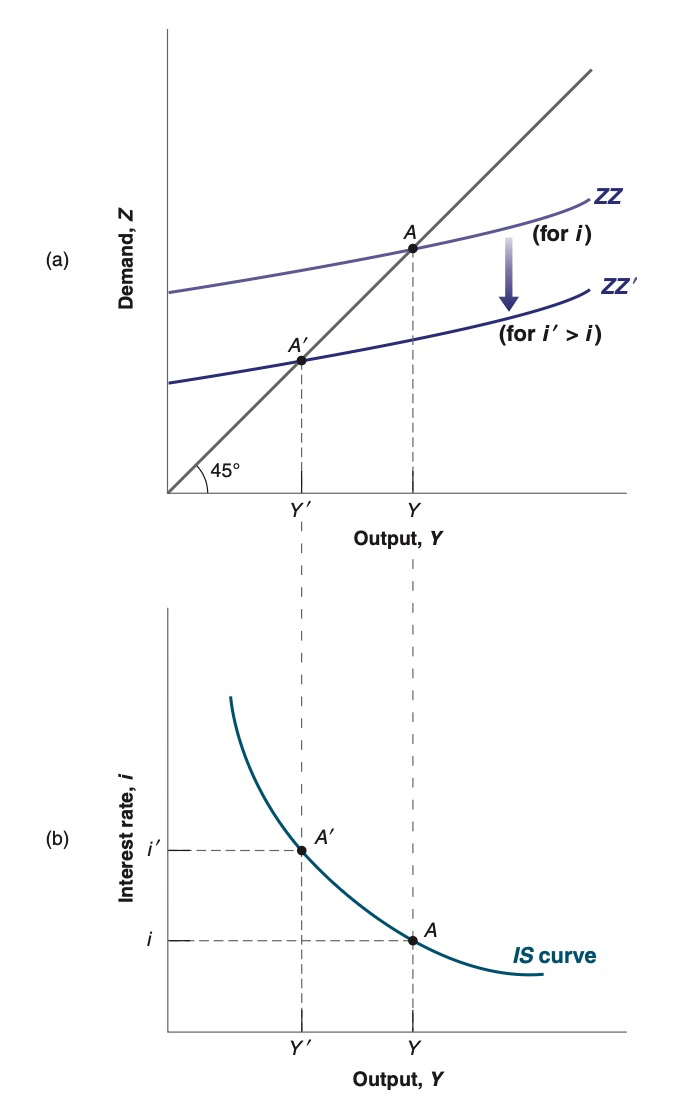
\includegraphics[width=\linewidth]{IS.png}
    \caption{Deriving IS Relation}
    \label{fig:IS}
  \end{minipage}%
  \hfill
  % Right side: text
  \begin{minipage}{0.6\linewidth}
    Recall from the equilibrium of Production = Demand, or equivalently Investment = Savings, we have:
    $$Z = C(Y-T) + \overline{I} + G$$

    Now, we'll build on this model and see how investment ($I$) is dependent on the interest rate ($i$). First though, investment is directly proportional on the level of sales ($Y$) because when people start buying more, production needs to increase, so a firm would invest in machines and the such to match the demand. Derivatives-wise, we would write this out as $ \frac{\partial I}{\partial Y} > 0$. Also, investment is inverseley proportional to the interest rate since an increase in the interest rate would mean the machines becomes more expensive, so firms are less likely to invest. Derivatives-wise, we write that as  $\frac{\partial I}{\partial i} < 0$. We then summarize this as:
    $$I = I(\underset{(+}{Y}, \underset{-)}{i})$$

    We now have the new and improved equation for demand as:
    $$Z = C(Y-T) + I(Y, i) + G$$

    Never forget the equilibrium of production equals demand, which is graphed out in (a). Here, we are seeing that as the interest rate increases from $i$ to $i'$, the demand curve shifts from $ZZ$ to $ZZ'$. We summarize all of this with the curve in (b) where as the interest rate increases, the output decreases. The IS relation and the IS curve show the combinations of the interest rate and the level of output that are consistent with equilibrium in the goods market. An increase in the interest rate leads to a decline in output. Consequently, the IS curve is downward sloping. Overall,
  \end{minipage}
\end{figure}


$$\Delta i^+ \underbrace{\implies}_{\frac{\partial I}{\partial i} < 0}  \Delta I^- \underbrace{\implies}_{Z = C + I + G} \Delta Z^- \underbrace{\implies}_{Y=Z} \Delta Y^-$$ 

\section{Financial Market \& LM Relation}
For the LM relation, we have the old and new way of thinking it. Of course, we'll be using the new, where we assume that the central bank chooses the interest rate $\overline{i}$. Thus, for any output $Y$, the central bank will do its expansionary and contractionary monetary operations so that the interest rate is $\overline{i}$.

To test your knowledge and understanding of the financial market, answer this question. The old way of thinking the LM relation was with an upwards curve where as output increases, the interest rate also increases. One key assumption in the old framework that does not hold anymore is that central banks fix the money supply (They don't anymore; they do their monetary operations happily.) Given this assumption of an unmoving money supply, how do we get an increasing relation between output ($Y$) and the interest rate ($i$). Hint is to look at the demand for money, $M^D = \$Y L(i)$ and what happens to the equilibrium in the financial market if there is an increase in real output ($Y$).
\section{Putting the Two Together - IS-LM Model}

\begin{figure}[H] 
  \centering % Left side: image 
  \begin{minipage}{0.4\linewidth} 
    \centering 
    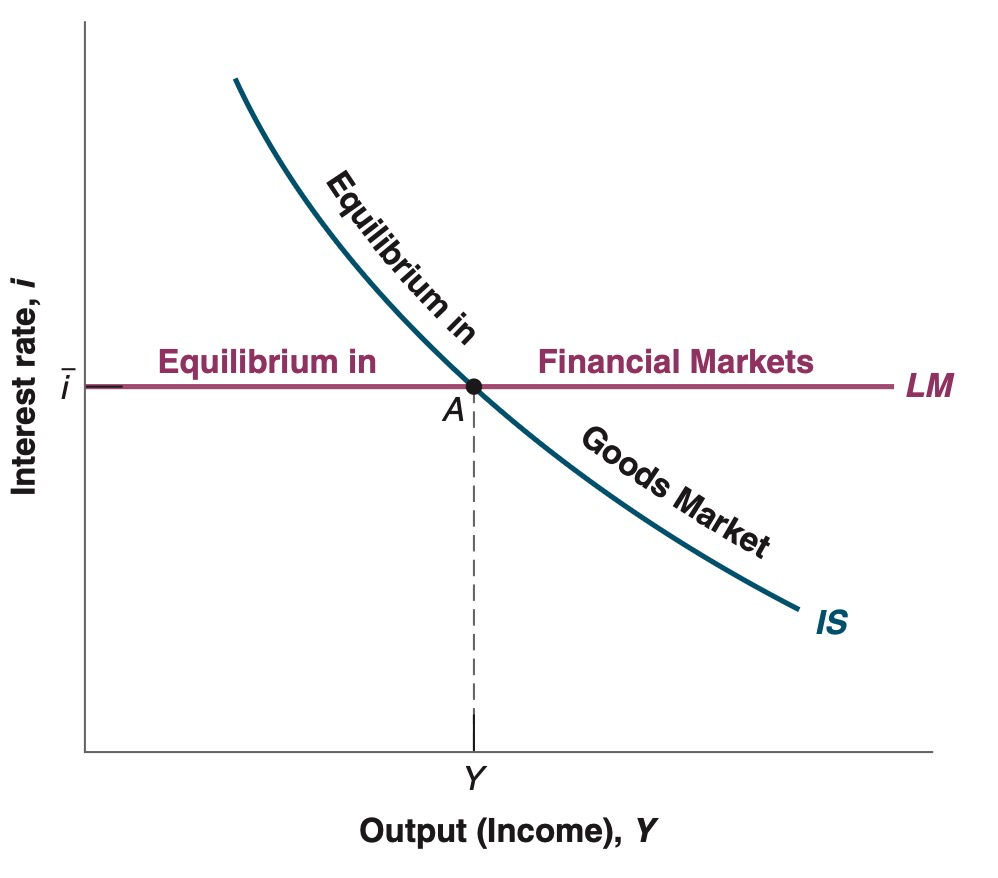
\includegraphics[width=\linewidth]{IS-LM.png} 
    \caption{The IS-LM Model} 
    \label{fig:IS-LM} 
  \end{minipage}% 
  % Right side: text 
  \begin{minipage}{0.6\linewidth} 
    We now put the the good and financial markets together, so we have: 
    \begin{align*} 
      \text{IS Relation: } Y &= C(Y-T) + I(Y, i) + G \\ 
      \text{LM Relation: } i &= \overline{i} 
    \end{align*} 
    Ideally, equilibrium is achieved in both markets at the intersection shown in Figure 2. From here, we can begin discussing fiscal and monetary policy, such as the effects of increased government spending or lower interest rates set by the central bank. To analyze these scenarios, we follow a three-step process, which we will also apply to examine the impact of a tax increase.
  \end{minipage} 
\end{figure}


\begin{enumerate}
  \item Does the event shift the IS curve and/or the LM curve, and, if so, how?
  \begin{enumerate}
    \item At all possible interest rates, an increase in taxes decreases output as shown by the chain of implications below:
    $$\Delta T^+ \implies \Delta(\text{Disposable Income})^- \implies \Delta C^- \implies \Delta Y^-$$
    Thus, the IS curve will shift to the left to show that output has decreased for all possible interest rates ($i$). For the LM curve, there is no shift since $\overline{i}$ is fixed by the central bank, NOT by the government.
  \end{enumerate}
  \item What does this event do to equilibrium output and the equilibrium interest rate?
  \begin{enumerate}
    \item Equilibrium output must decrease while equilibrium interest rate is the same as shown in Figure \ref{fig:shift}.
  \begin{figure}[h]
    \centering
    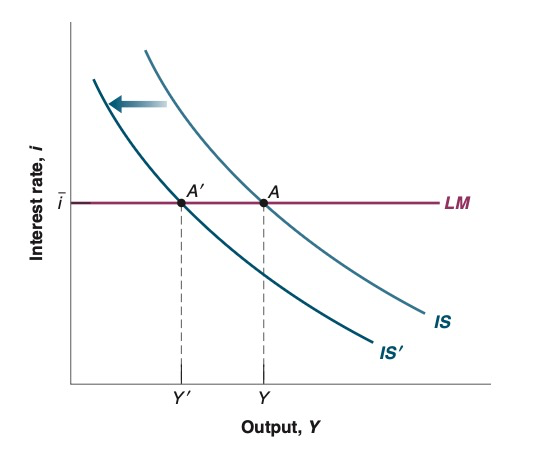
\includegraphics[width=0.4\linewidth]{shift-IS.png}
    \caption{The Effects of an Increase in Taxes}
    \label{fig:shift}
  \end{figure}

  \end{enumerate}
  \item Describe the effects in words. 
  \begin{enumerate}
    \item We leave this an exercise to the reader.
  \end{enumerate}
\end{enumerate}

As a short summary, a fiscal expansion shifts the IS curve to the right, leading to an increase in output. A fiscal contraction shifts the IS curve to the left, leading to a decrease in output. On the other hand, a monetary expansion shifts the LM curve down, leading to a decrease in the interest rate and an increase in output. A monetary contraction shifts the LM curve up, leading to an increase in the interest rate and a decrease in output.

The combination of monetary and fiscal policies is known as the monetary-fiscal policy mix, or simply the policy mix. Sometimes monetary and fiscal policy are used in the same direction, sometimes in opposite directions. Together, a fiscal contraction and a monetary expansion can, for example, achieve a decrease in the budget deficit while avoiding a decrease in output
\section{Time Dynamics of the IS-LM Model}
The IS-LM model appears to describe well the behavior of the economy in the short run. In particular, the effects of monetary policy are similar to those implied by the IS-LM model once dynamics are introduced in the model. An increase in the interest rate due to a monetary contraction leads to a decrease in output, with the maximum ­ effect taking place after about eight quarters. 

It also shows the assumption that prices are sticky because the price level is nearly unchanged
for the first six quarters or so. Only after the first six quarters does it decline. This
gives us a strong hint as to why the IS-LM model becomes less reliable as we look at
the medium run: In the medium run, we can no longer assume that the price level is
given, and movements in the price level become important.
\end{document}